\documentclass{article}%
\usepackage[T1]{fontenc}%
\usepackage[utf8]{inputenc}%
\usepackage{lmodern}%
\usepackage{textcomp}%
\usepackage{lastpage}%
\usepackage{geometry}%
\usepackage{tabularx}%
\usepackage{booktabs}%
\usepackage[dvipsnames]{xcolor}
\usepackage{tikz}
\usepackage{tkz-graph}
\usepackage{tkz-berge}
\usetikzlibrary{arrows,shapes}
\usepackage[matrix,arrow,curve,cmtip]{xy}
\usepackage{svg}
\usepackage{multicol}
\usepackage{float}
\usepackage{graphicx}
\usepackage[shortlabels]{enumitem}
\geometry{tmargin=2cm,lmargin=2cm,rmargin=2cm,bmargin=2cm}%
%
%
%
\definecolor{red0}{rgb}{1.0,0,0}
\definecolor{red1}{rgb}{0.92,0,0}
\definecolor{red2}{rgb}{0.84,0,0}
\definecolor{red3}{rgb}{0.76,0,0}
\definecolor{red4}{rgb}{0.6799999999999999,0,0}
\definecolor{red5}{rgb}{0.6,0,0}
\definecolor{red6}{rgb}{0.52,0,0}
\definecolor{red7}{rgb}{0.43999999999999995,0,0}
\definecolor{red8}{rgb}{0.36,0,0}
\definecolor{red9}{rgb}{0.28,0,0}
\definecolor{green0}{rgb}{0,1.0,0}
\definecolor{green1}{rgb}{0,0.9272727272727272,0}
\definecolor{green2}{rgb}{0,0.8545454545454545,0}
\definecolor{green3}{rgb}{0,0.7818181818181817,0}
\definecolor{green4}{rgb}{0,0.709090909090909,0}
\definecolor{green5}{rgb}{0,0.6363636363636362,0}
\definecolor{green6}{rgb}{0,0.5636363636363636,0}
\definecolor{green7}{rgb}{0,0.49090909090909085,0}
\definecolor{green8}{rgb}{0,0.4181818181818181,0}
\definecolor{green9}{rgb}{0,0.34545454545454535,0}
\definecolor{green10}{rgb}{0,0.2727272727272726,0}
%
%
%
\title{Test dataset}

\author{Christopher-Lloyd Simon and Ben Stucky}

\begin{document}%
\maketitle
\small

\section{$7\_6$}

\begin{multicols}{2}
{\normalsize \noindent\textbf{Total optimal pinning sets:} 1

\noindent\textbf{Total minimal pinning sets:} 3

\noindent\textbf{Total pinning sets:} 44

\noindent\textbf{Pinning number:} 4

}
\columnbreak

{\normalsize \noindent\textbf{Average optimal gonality:} 2.25

\noindent\textbf{Average minimal gonality:} 2.42

\noindent\textbf{Average overall gonality:} 2.82

}
\end{multicols}

\begin{table}[ht]
	\caption{Pinning sets/average gonality by cardinal}
	\centering
	\renewcommand{\arraystretch}{1.5}
	\begin{tabularx}{\textwidth}{lXXXXXXXX}
		\toprule
			Cardinal & 4 & 5 & 6 & 7 & 8 & 9 & Total\\
			\hline
			Optimal pinning sets & 1 & 0 & 0 & 0 & 0 & 0 & 1 \\
			Minimal (suboptimal) pinning sets & 0 & 2 & 0 & 0 & 0 & 0 & 2 \\
			Nonminimal pinning sets & 0 & 5 & 15 & 14 & 6 & 1 & 41 \\
			Average gonality & 2.25 & 2.54 & 2.78 & 2.94 & 3.04 & 3.11 &  \\
		\bottomrule \\ 
	\end{tabularx}
\end{table}

\begin{table}[ht]
	\caption{Pinning set data}
	\centering
	\renewcommand{\arraystretch}{1.5}
	\begin{tabularx}{\textwidth}{lXXXXXX}
		\toprule
			Pinning set & Pindicator & Regions & Card & Gonality seq & Average gonality\\
			\hline
			A (optimal) & {\Huge\textcolor{red0}{\textbullet}} & $\{1,3,4,8\}$ & 4 & [2, 3, 2, 2] & 2.25 \\
			a (minimal) & {\Huge\textcolor{green0}{\textbullet}} & $\{1,2,4,7,8\}$ & 5 & [2, 3, 2, 3, 2] & 2.4 \\
			b (minimal) & {\Huge\textcolor{green5}{\textbullet}} & $\{1,2,4,6,8\}$ & 5 & [2, 3, 2, 4, 2] & 2.6 \\
		\bottomrule \\ 
	\end{tabularx}
\end{table}

\newpage

\begin{multicols}{2}
\begin{figure}[H]
\centering
\def\svgscale{0.7}
\includesvg{tex/img/7_6.svg}
\caption{Snappy loop plot.}
\label{fig:tex/img/7_6.svg}
\end{figure}
\columnbreak

\begin{figure}[H]
\centering
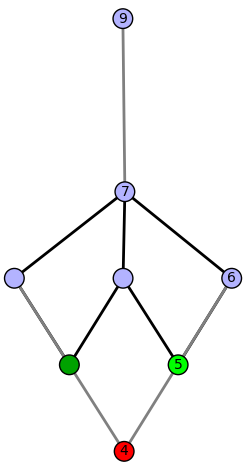
\includegraphics[scale=.9]{tex/img/7_6.png}
\caption{Minimal join semilattice of pinning sets.}
\label{fig:tex/img/7_6.png}
\end{figure}
\end{multicols}

\newpage

\section{[(1, 7, 2, 6), (4, 9, 5, 10), (2, 12, 3, 11), (7, 13, 8, 12), (18, 13, 1, 14), (3, 17, 4, 16), (5, 14, 6, 15), (8, 18, 9, 17), (10, 15, 11, 16)]}

\begin{multicols}{2}
{\normalsize \noindent\textbf{Total optimal pinning sets:} 2

\noindent\textbf{Total minimal pinning sets:} 13

\noindent\textbf{Total pinning sets:} 395

\noindent\textbf{Pinning number:} 4

}
\columnbreak

{\normalsize \noindent\textbf{Average optimal gonality:} 3.0

\noindent\textbf{Average minimal gonality:} 3.25

\noindent\textbf{Average overall gonality:} 3.23

}
\end{multicols}

\begin{table}[ht]
	\caption{Pinning sets/average gonality by cardinal}
	\centering
	\renewcommand{\arraystretch}{1.5}
	\begin{tabularx}{\textwidth}{lXXXXXXXXXX}
		\toprule
			Cardinal & 4 & 5 & 6 & 7 & 8 & 9 & 10 & 11 & Total\\
			\hline
			Optimal pinning sets & 2 & 0 & 0 & 0 & 0 & 0 & 0 & 0 & 2 \\
			Minimal (suboptimal) pinning sets & 0 & 4 & 7 & 0 & 0 & 0 & 0 & 0 & 11 \\
			Nonminimal pinning sets & 0 & 14 & 66 & 130 & 111 & 49 & 11 & 1 & 382 \\
			Average gonality & 3.0 & 3.13 & 3.21 & 3.23 & 3.25 & 3.27 & 3.27 & 3.27 &  \\
		\bottomrule \\ 
	\end{tabularx}
\end{table}

\begin{table}[ht]
	\caption{Pinning set data}
	\centering
	\renewcommand{\arraystretch}{1.5}
	\begin{tabularx}{\textwidth}{lXXXXXX}
		\toprule
			Pinning set & Pindicator & Regions & Card & Gonality seq & Average gonality\\
			\hline
			A (optimal) & {\Huge\textcolor{red0}{\textbullet}} & $\{2,6,9,10\}$ & 4 & [3, 3, 3, 3] & 3.0 \\
			B (optimal) & {\Huge\textcolor{red5}{\textbullet}} & $\{1,3,4,8\}$ & 4 & [3, 3, 3, 3] & 3.0 \\
			a (minimal) & {\Huge\textcolor{green0}{\textbullet}} & $\{2,4,6,8,11\}$ & 5 & [3, 3, 3, 3, 4] & 3.2 \\
			b (minimal) & {\Huge\textcolor{green1}{\textbullet}} & $\{2,5,7,8,11\}$ & 5 & [3, 4, 4, 3, 4] & 3.6 \\
			c (minimal) & {\Huge\textcolor{green2}{\textbullet}} & $\{1,2,5,8,9\}$ & 5 & [3, 3, 4, 3, 3] & 3.2 \\
			d (minimal) & {\Huge\textcolor{green3}{\textbullet}} & $\{2,3,7,8,10\}$ & 5 & [3, 3, 4, 3, 3] & 3.2 \\
			e (minimal) & {\Huge\textcolor{green4}{\textbullet}} & $\{2,6,7,8,10,11\}$ & 6 & [3, 3, 4, 3, 3, 4] & 3.33 \\
			f (minimal) & {\Huge\textcolor{green5}{\textbullet}} & $\{2,5,6,8,9,11\}$ & 6 & [3, 4, 3, 3, 3, 4] & 3.33 \\
			g (minimal) & {\Huge\textcolor{green6}{\textbullet}} & $\{2,5,7,8,9,10\}$ & 6 & [3, 4, 4, 3, 3, 3] & 3.33 \\
			h (minimal) & {\Huge\textcolor{green7}{\textbullet}} & $\{1,2,4,5,8,11\}$ & 6 & [3, 3, 3, 4, 3, 4] & 3.33 \\
			i (minimal) & {\Huge\textcolor{green8}{\textbullet}} & $\{1,3,4,6,9,10\}$ & 6 & [3, 3, 3, 3, 3, 3] & 3.0 \\
			j (minimal) & {\Huge\textcolor{green9}{\textbullet}} & $\{2,3,4,7,8,11\}$ & 6 & [3, 3, 3, 4, 3, 4] & 3.33 \\
			k (minimal) & {\Huge\textcolor{green10}{\textbullet}} & $\{1,2,3,5,7,8\}$ & 6 & [3, 3, 3, 4, 4, 3] & 3.33 \\
		\bottomrule \\ 
	\end{tabularx}
\end{table}

\newpage

\begin{multicols}{2}
\begin{figure}[H]
\centering
\def\svgscale{0.7}
\includesvg{tex/img/[(1, 7, 2, 6), (4, 9, 5, 10), (2, 12, 3, 11), (7, 13, 8, 12), (18, 13, 1, 14), (3, 17, 4, 16), (5, 14, 6, 15), (8, 18, 9, 17), (10, 15, 11, 16)].svg}
\caption{Snappy loop plot.}
\label{fig:tex/img/[(1, 7, 2, 6), (4, 9, 5, 10), (2, 12, 3, 11), (7, 13, 8, 12), (18, 13, 1, 14), (3, 17, 4, 16), (5, 14, 6, 15), (8, 18, 9, 17), (10, 15, 11, 16)].svg}
\end{figure}
\columnbreak

\begin{figure}[H]
\centering
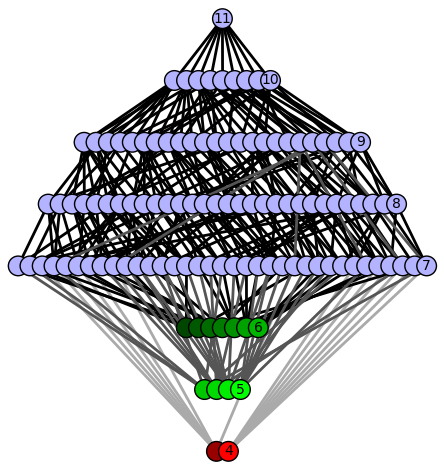
\includegraphics[scale=.9]{tex/img/[(1, 7, 2, 6), (4, 9, 5, 10), (2, 12, 3, 11), (7, 13, 8, 12), (18, 13, 1, 14), (3, 17, 4, 16), (5, 14, 6, 15), (8, 18, 9, 17), (10, 15, 11, 16)].png}
\caption{Minimal join semilattice of pinning sets.}
\label{fig:tex/img/[(1, 7, 2, 6), (4, 9, 5, 10), (2, 12, 3, 11), (7, 13, 8, 12), (18, 13, 1, 14), (3, 17, 4, 16), (5, 14, 6, 15), (8, 18, 9, 17), (10, 15, 11, 16)].png}
\end{figure}
\end{multicols}

\newpage

\section{[(1, 7, 2, 6), (3, 8, 4, 9), (5, 11, 6, 10), (16, 12, 1, 11), (2, 13, 3, 14), (4, 16, 5, 15), (7, 12, 8, 13), (9, 15, 10, 14)]}

\begin{multicols}{2}
{\normalsize \noindent\textbf{Total optimal pinning sets:} 10

\noindent\textbf{Total minimal pinning sets:} 10

\noindent\textbf{Total pinning sets:} 160

\noindent\textbf{Pinning number:} 5

}
\columnbreak

{\normalsize \noindent\textbf{Average optimal gonality:} 3.04

\noindent\textbf{Average minimal gonality:} 3.04

\noindent\textbf{Average overall gonality:} 3.15

}
\end{multicols}

\begin{table}[ht]
	\caption{Pinning sets/average gonality by cardinal}
	\centering
	\renewcommand{\arraystretch}{1.5}
	\begin{tabularx}{\textwidth}{lXXXXXXXX}
		\toprule
			Cardinal & 5 & 6 & 7 & 8 & 9 & 10 & Total\\
			\hline
			Optimal pinning sets & 10 & 0 & 0 & 0 & 0 & 0 & 10 \\
			Minimal (suboptimal) pinning sets & 0 & 0 & 0 & 0 & 0 & 0 & 0 \\
			Nonminimal pinning sets & 0 & 42 & 60 & 37 & 10 & 1 & 150 \\
			Average gonality & 3.04 & 3.11 & 3.16 & 3.19 & 3.2 & 3.2 &  \\
		\bottomrule \\ 
	\end{tabularx}
\end{table}

\begin{table}[ht]
	\caption{Pinning set data}
	\centering
	\renewcommand{\arraystretch}{1.5}
	\begin{tabularx}{\textwidth}{lXXXXXX}
		\toprule
			Pinning set & Pindicator & Regions & Card & Gonality seq & Average gonality\\
			\hline
			A (optimal) & {\Huge\textcolor{red0}{\textbullet}} & $\{1,3,5,7,9\}$ & 5 & [3, 3, 3, 3, 3] & 3.0 \\
			B (optimal) & {\Huge\textcolor{red1}{\textbullet}} & $\{1,3,5,8,10\}$ & 5 & [3, 3, 3, 3, 4] & 3.2 \\
			C (optimal) & {\Huge\textcolor{red2}{\textbullet}} & $\{1,3,4,7,8\}$ & 5 & [3, 3, 3, 3, 3] & 3.0 \\
			D (optimal) & {\Huge\textcolor{red3}{\textbullet}} & $\{1,3,4,7,9\}$ & 5 & [3, 3, 3, 3, 3] & 3.0 \\
			E (optimal) & {\Huge\textcolor{red4}{\textbullet}} & $\{2,4,5,8,9\}$ & 5 & [3, 3, 3, 3, 3] & 3.0 \\
			F (optimal) & {\Huge\textcolor{red5}{\textbullet}} & $\{2,4,6,7,9\}$ & 5 & [3, 3, 4, 3, 3] & 3.2 \\
			G (optimal) & {\Huge\textcolor{red6}{\textbullet}} & $\{2,3,5,8,9\}$ & 5 & [3, 3, 3, 3, 3] & 3.0 \\
			H (optimal) & {\Huge\textcolor{red7}{\textbullet}} & $\{2,3,5,7,9\}$ & 5 & [3, 3, 3, 3, 3] & 3.0 \\
			I (optimal) & {\Huge\textcolor{red8}{\textbullet}} & $\{1,2,4,7,8\}$ & 5 & [3, 3, 3, 3, 3] & 3.0 \\
			J (optimal) & {\Huge\textcolor{red9}{\textbullet}} & $\{1,2,4,5,8\}$ & 5 & [3, 3, 3, 3, 3] & 3.0 \\
		\bottomrule \\ 
	\end{tabularx}
\end{table}

\newpage

\begin{multicols}{2}
\begin{figure}[H]
\centering
\def\svgscale{0.7}
\includesvg{tex/img/[(1, 7, 2, 6), (3, 8, 4, 9), (5, 11, 6, 10), (16, 12, 1, 11), (2, 13, 3, 14), (4, 16, 5, 15), (7, 12, 8, 13), (9, 15, 10, 14)].svg}
\caption{Snappy loop plot.}
\label{fig:tex/img/[(1, 7, 2, 6), (3, 8, 4, 9), (5, 11, 6, 10), (16, 12, 1, 11), (2, 13, 3, 14), (4, 16, 5, 15), (7, 12, 8, 13), (9, 15, 10, 14)].svg}
\end{figure}
\columnbreak

\begin{figure}[H]
\centering
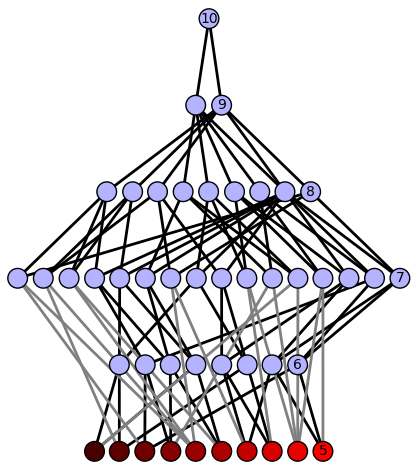
\includegraphics[scale=.9]{tex/img/[(1, 7, 2, 6), (3, 8, 4, 9), (5, 11, 6, 10), (16, 12, 1, 11), (2, 13, 3, 14), (4, 16, 5, 15), (7, 12, 8, 13), (9, 15, 10, 14)].png}
\caption{Minimal join semilattice of pinning sets.}
\label{fig:tex/img/[(1, 7, 2, 6), (3, 8, 4, 9), (5, 11, 6, 10), (16, 12, 1, 11), (2, 13, 3, 14), (4, 16, 5, 15), (7, 12, 8, 13), (9, 15, 10, 14)].png}
\end{figure}
\end{multicols}

\newpage


\end{document}